%%
%% This is file `sample-authordraft.tex',
%% generated with the docstrip utility.
%%
%% The original source files were:
%%
%% samples.dtx  (with options: `authordraft')
%% 
%% IMPORTANT NOTICE:
%% 
%% For the copyright see the source file.
%% 
%% Any modified versions of this file must be renamed
%% with new filenames distinct from sample-authordraft.tex.
%% 
%% For distribution of the original source see the terms
%% for copying and modification in the file samples.dtx.
%% 
%% This generated file may be distributed as long as the
%% original source files, as listed above, are part of the
%% same distribution. (The sources need not necessarily be
%% in the same archive or directory.)
%%
%% The first command in your LaTeX source must be the \documentclass command.
\documentclass[sigconf]{acmart}

%%
%% \BibTeX command to typeset BibTeX logo in the docs
\AtBeginDocument{%
  \providecommand\BibTeX{{%
    \normalfont B\kern-0.5em{\scshape i\kern-0.25em b}\kern-0.8em\TeX}}}

%% Rights management information.  This information is sent to you
%% when you complete the rights form.  These commands have SAMPLE
%% values in them; it is your responsibility as an author to replace
%% the commands and values with those provided to you when you
%% complete the rights form.
\setcopyright{rightsretained}
\copyrightyear{2021}
\acmYear{2021}
\acmDOI{CS460.org}

%% These commands are for a PROCEEDINGS abstract or paper.
\acmConference[CS460]{CS460: Computer Graphics at UMass Boston}{Fall 2021}{Boston, MA}
\acmBooktitle{CS460: Computer Graphics at UMass Boston, Fall 2021}
\acmPrice{1.00}
\acmISBN{1337}


%%
%% Submission ID.
%% Use this when submitting an article to a sponsored event. You'll
%% receive a unique submission ID from the organizers
%% of the event, and this ID should be used as the parameter to this command.
%%\acmSubmissionID{123-A56-BU3}

%%
%% The majority of ACM publications use numbered citations and
%% references.  The command \citestyle{authoryear} switches to the
%% "author year" style.
%%
%% If you are preparing content for an event
%% sponsored by ACM SIGGRAPH, you must use the "author year" style of
%% citations and references.
%% Uncommenting
%% the next command will enable that style.
%%\citestyle{acmauthoryear}

%%
%% end of the preamble, start of the body of the document source.
\begin{document}

%%
%% The "title" command has an optional parameter,
%% allowing the author to define a "short title" to be used in page headers.
\title{SOMETHING IN THE WOOD}

%%
%% The "author" command and its associated commands are used to define
%% the authors and their affiliations.
%% Of note is the shared affiliation of the first two authors, and the
%% "authornote" and "authornotemark" commands
%% used to denote shared contribution to the research.
\author{Duy Anh Nguyen}
\email{DuyAnh.Nguyen001@umb.edu}
\affiliation{%
  \institution{University of Massachusetts Boston}
}


%%
%% By default, the full list of authors will be used in the page
%% headers. Often, this list is too long, and will overlap
%% other information printed in the page headers. This command allows
%% the author to define a more concise list
%% of authors' names for this purpose.
\renewcommand{\shortauthors}{}

%%
%% The abstract is a short summary of the work to be presented in the
%% article.
\begin{abstract}
  "Something in the Wood" is an independent FPS game created using Unity Engine. The game is a product that aims to recreate some of the most important aspects that most AAA FPS games should have. The game has an in-depth control system such as gun switching using the mouse scroll wheel, each weapon having different functionality, zoom in and zoom out for accurate aim, and as well as simple action such as sprinting and shooting similarly to other FPS games. 
\end{abstract}

%%
%% Keywords. The author(s) should pick words that accurately describe
%% the work being presented. Separate the keywords with commas.
\keywords{Unity, Unity Asset Store, Visualization, Graphic}

%% A "teaser" image appears between the author and affiliation
%% information and the body of the document, and typically spans the
%% page.
\begin{teaserfigure}
  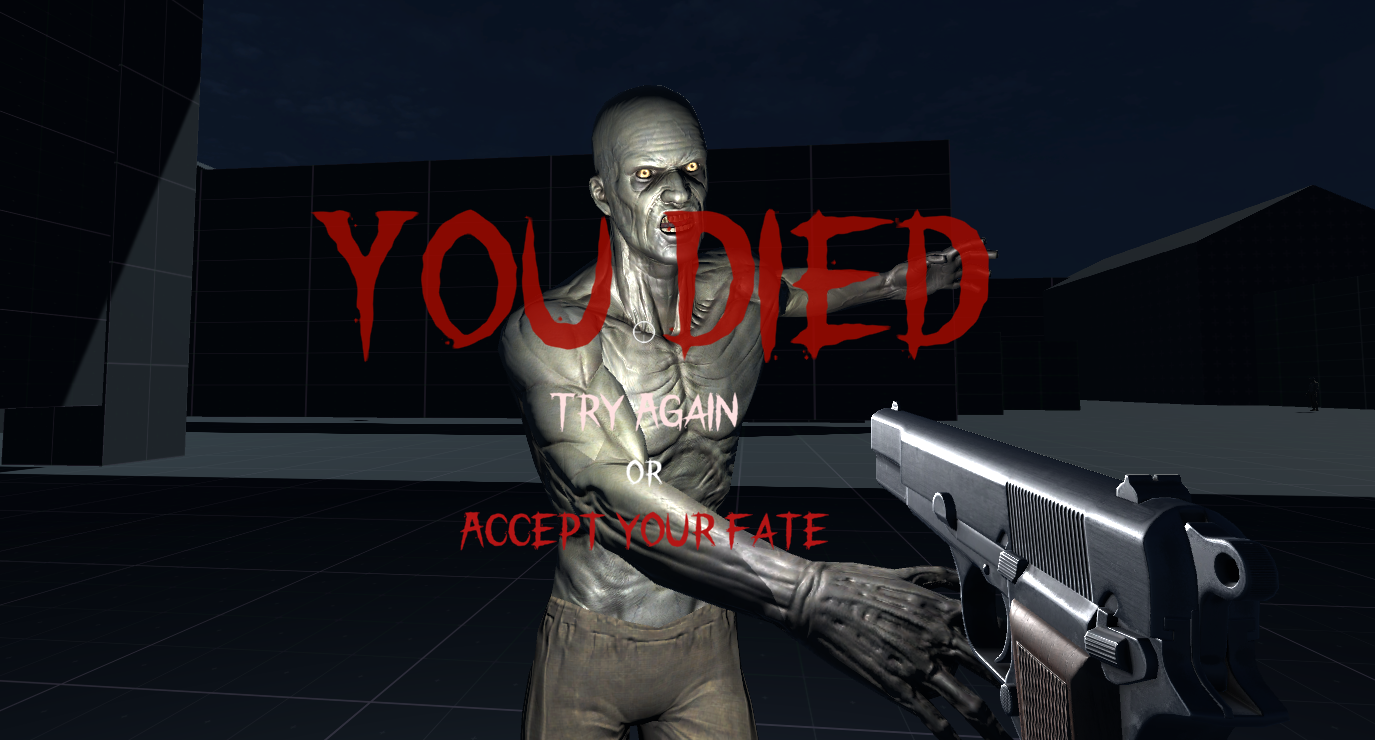
\includegraphics[width=\textwidth]{gfx/wood.png}
  \caption{Add a nice wide figure here and replace this caption.}
  \label{fig:teaser}
\end{teaserfigure}

%%
%% This command processes the author and affiliation and title
%% information and builds the first part of the formatted document.
\maketitle

\section{Introduction}

I have used Unity as an Engine to create a 3D-Fighting game called "Project Strike" before, I was the happy result but in that project, I have made some fundamental mistakes that a game developer should avoid. "Something in the Wood" is my second attempt of transferring my creativty into experience, at the same time a chance to correct the mistakes that I made from my previous projects.

\section{Related Work}

I took an inspiration from my last game, "Project Strike" an 3D Fighting game create by me and my friend The Phong using Unity~\cite{XTK} and Mixamo~\cite{Threejs}.

\section{Method}

Upon starting to create this project, I tried to set up milestones that I need to complete at the end of the project. The first thing and the most important that every game should have is an interactive and smooth control system, even though a control system is not the first thing that a player can see the first time they experience any game, but a smooth control system can keep the player sitting on the couch for hours. To do this I use a script provided by the Unity Standard Assets, attached that script to the Main Camera component. Once the basic of a game controller is completed, I developed an AI system that allows the enemy to follow the player if the player enters a certain range that the AI can see at the same time game the AI some different functionality and animation depend on the current state of the AI.

\subsection{Implementation}
%  The most importatnt aspect of every FPS game is that you as a player should be able to shoot.
 Code for implementation of Weapon script, the most common aspect of every FPS game
\begin{verbatim}

private void ProcessRaycast()
{
    RaycastHit hit;
    if (Physics.Raycast(FPCamera.transform.position,
    FPCamera.transform.forward, out hit, range))
    {
        CreateHitImpact(hit);
        EnemyHealth target = 
        hit.transform.GetComponent<EnemyHealth>();
        if (target == null) return;
        target.TakeDamage(damage);
    }
    else
    {
        return;
    }
}
\end{verbatim}

\subsection{Milestones}


\subsubsection{Milestone 1}

An example could be: I brained storm the concept for my FPS, what kind of setting that I would like to have in my world, what tool should I used to implemented it. 

\subsubsection{Milestone 2}

An example could be: At the end I decided to create an FPS horror game using Unity Engine since Unity Engine is created to make game, it would make the progress of making my game become easier than using Three.js alone.

\subsubsection{Milestone 3}

Start implementing the prototype of an FPS controller using existing FPS controller on the unity asset store as a model

\subsubsection{Milestone 4}

Start implementing the core system of an AI in a horror game, include action such as engage, attack, idle and follow.

\subsubsection{Milestone 5}

Creating functionality for decreasing health of the player and health of the AI whenever each of the target is being attack.

\subsubsection{Milestone 6}

Start create UI for the game. Death menu, Start menu, crosshair for player aim, zoom in and out system for some weapon.

\subsubsection{Milestone 6}

Creating animation for the AI, for example death, run, attack and idle animation.

\subsubsection{Milestone 7}

Level design, creating terrain and tree to create a horror atmosphere.

\subsection{Challenges}

\begin{itemize}
    \item Challenge 1: Switching the weapon using the mouse scroll wheel.
    \item Challenge 2: Making the AI rotate according to the player's position.
    \item Challenge 3: Zoom bug changing weapon while zoomed will keep the zoom for subsequent weapons.
    \item Challenge 4: Enemy will keep moving if they are dead.
    \item Challenge 5: Creating each different ammo for corresponding gun.
    \item Challenge 6: Player can still move even if the game is over.
    \item Challenge 7: Player rotation speed does not change even if the weapon is in zoom mode.
    
\end{itemize}

\section{Results}

The result of this project is exactly what I had it my mine when I was in the brainstormed phase of the project. I successfully completed all the goal that I have set out from the start of this project during the fast forward presentation, starting from smooth controller, variety of weapon and different type of enemies. 

\begin{figure}[h]
  \centering
  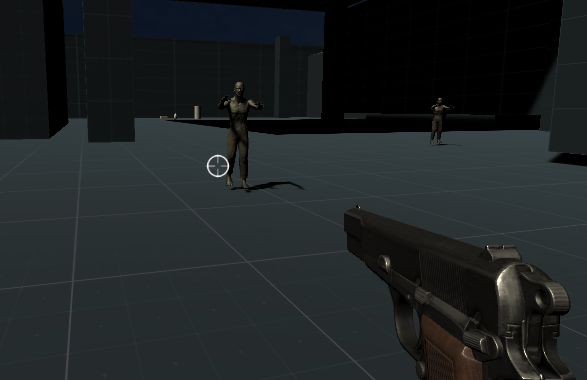
\includegraphics[width=\linewidth]{gfx/wood3.png}
  \caption{Enemy chase state}
  \label{fig:example}
\end{figure}


% You could also use a table like this:
%
\begin{table}

  \caption{Table 1: Game Performance}
  \label{tab:example}
  \begin{tabular}{ccl}
    \toprule
    Device & Performance \\ % header
    \midrule
    PC & 60 FPS \\ 
    Macbook & 60 FPS \\
    \bottomrule
  \end{tabular}
\end{table}

\section{Conclusions}

This is one of the most interesting projects that I have done for a while because of the complexity that needs to be done to give the player a good experience, even though there is a lot of polish and level design that still needs to be done after the submission of the Final Project report. As well as some export methods need to be done by using Unity Functionality to be accessed and played with WebGL. 

%%
%% REFERENCES
%%
\bibliographystyle{ACM-Reference-Format}

\bibliography{references}

\end{document}
\endinput
